\apendice{Especificación de diseño}

\section{Introducción}
En este apartado se va a explicar el análisis y diseño de los datos. También se va a exponer cómo se han resuelto las especificaciones y los casos de uso mencionados en el apartado anterior.  

Uno de los objetivos de este apartado es la comprensión  de la toma de decisiones y los motivos o causas que han dado lugar a las mismas.

\section{Diseño de datos}


\subsection{Modelo Entidad-Relación(ER)}
A continuación en la figura \ref{fig:ModeloER} se observa el modelo ER o Diagrama Relacional de la Base de Datos de la aplicación.


\begin{figure}%[!h]
		\centering
		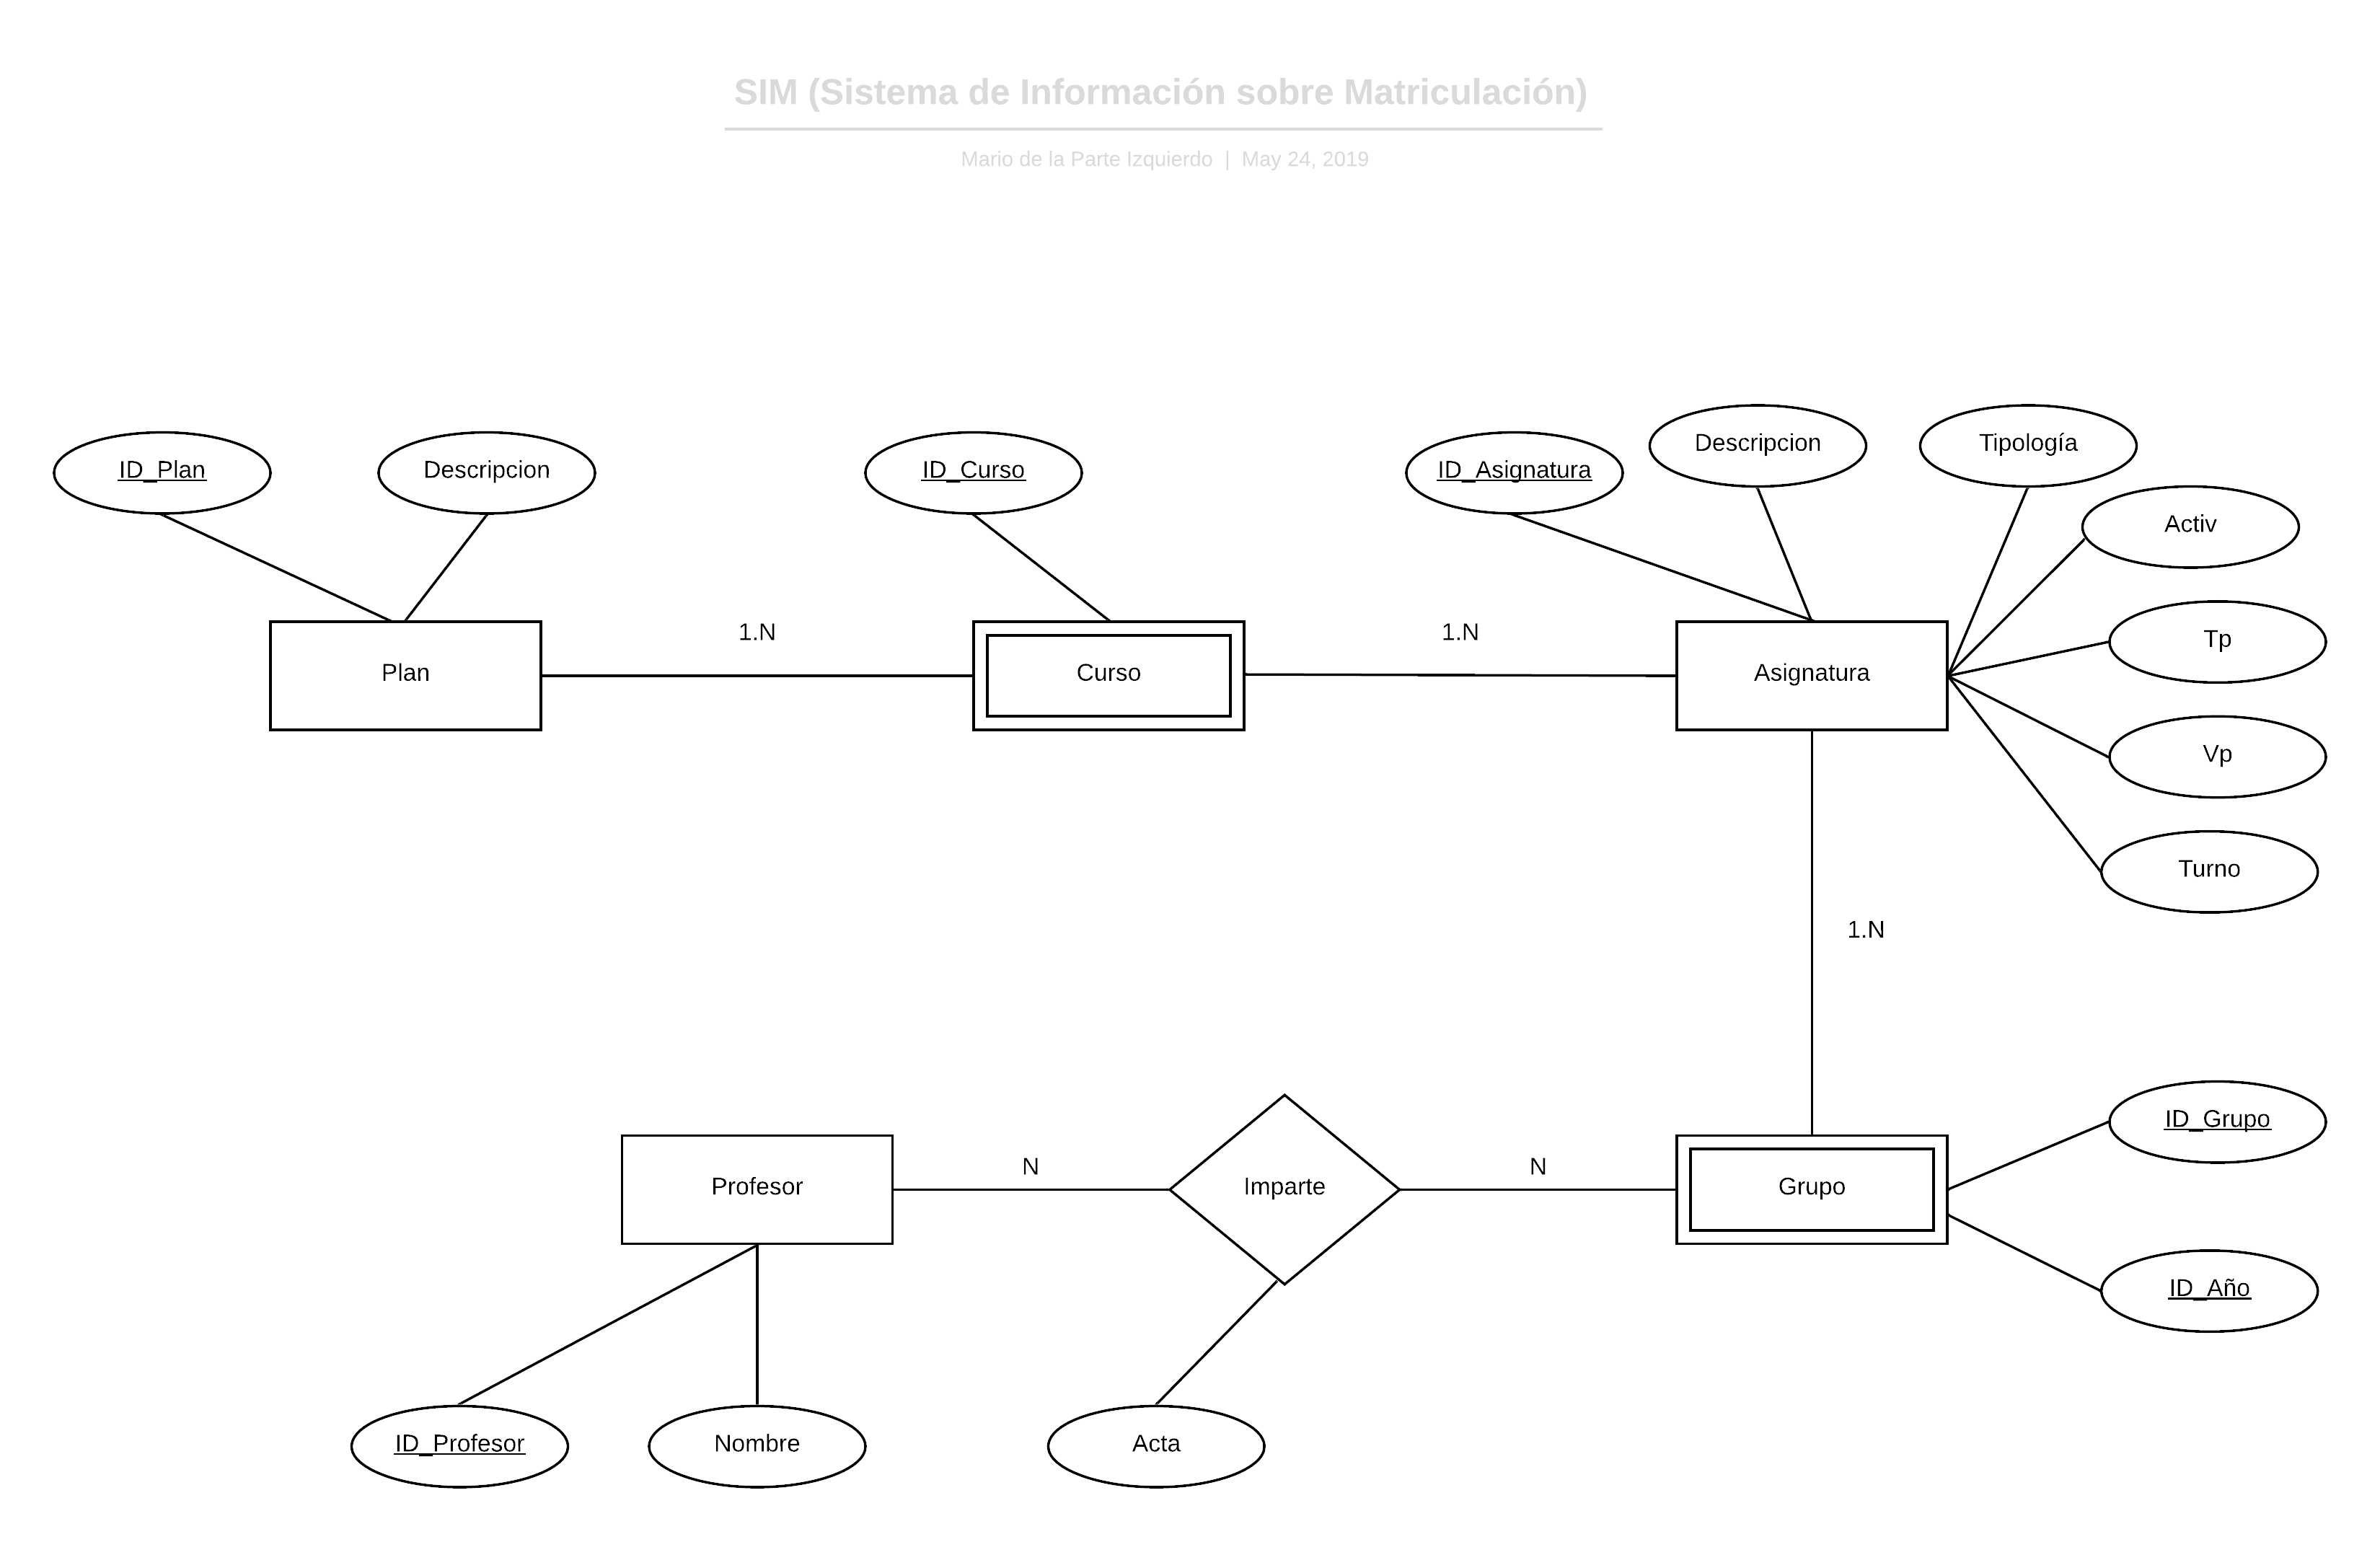
\includegraphics[angle=90, width=\textwidth]{ModeloER}
		\caption{Modelo Entidad-Relación(ER)}\label{fig:ModeloER}
	\end{figure}

% \imagen{ModeloER}{Modelo Entidad-Relación(ER)}
%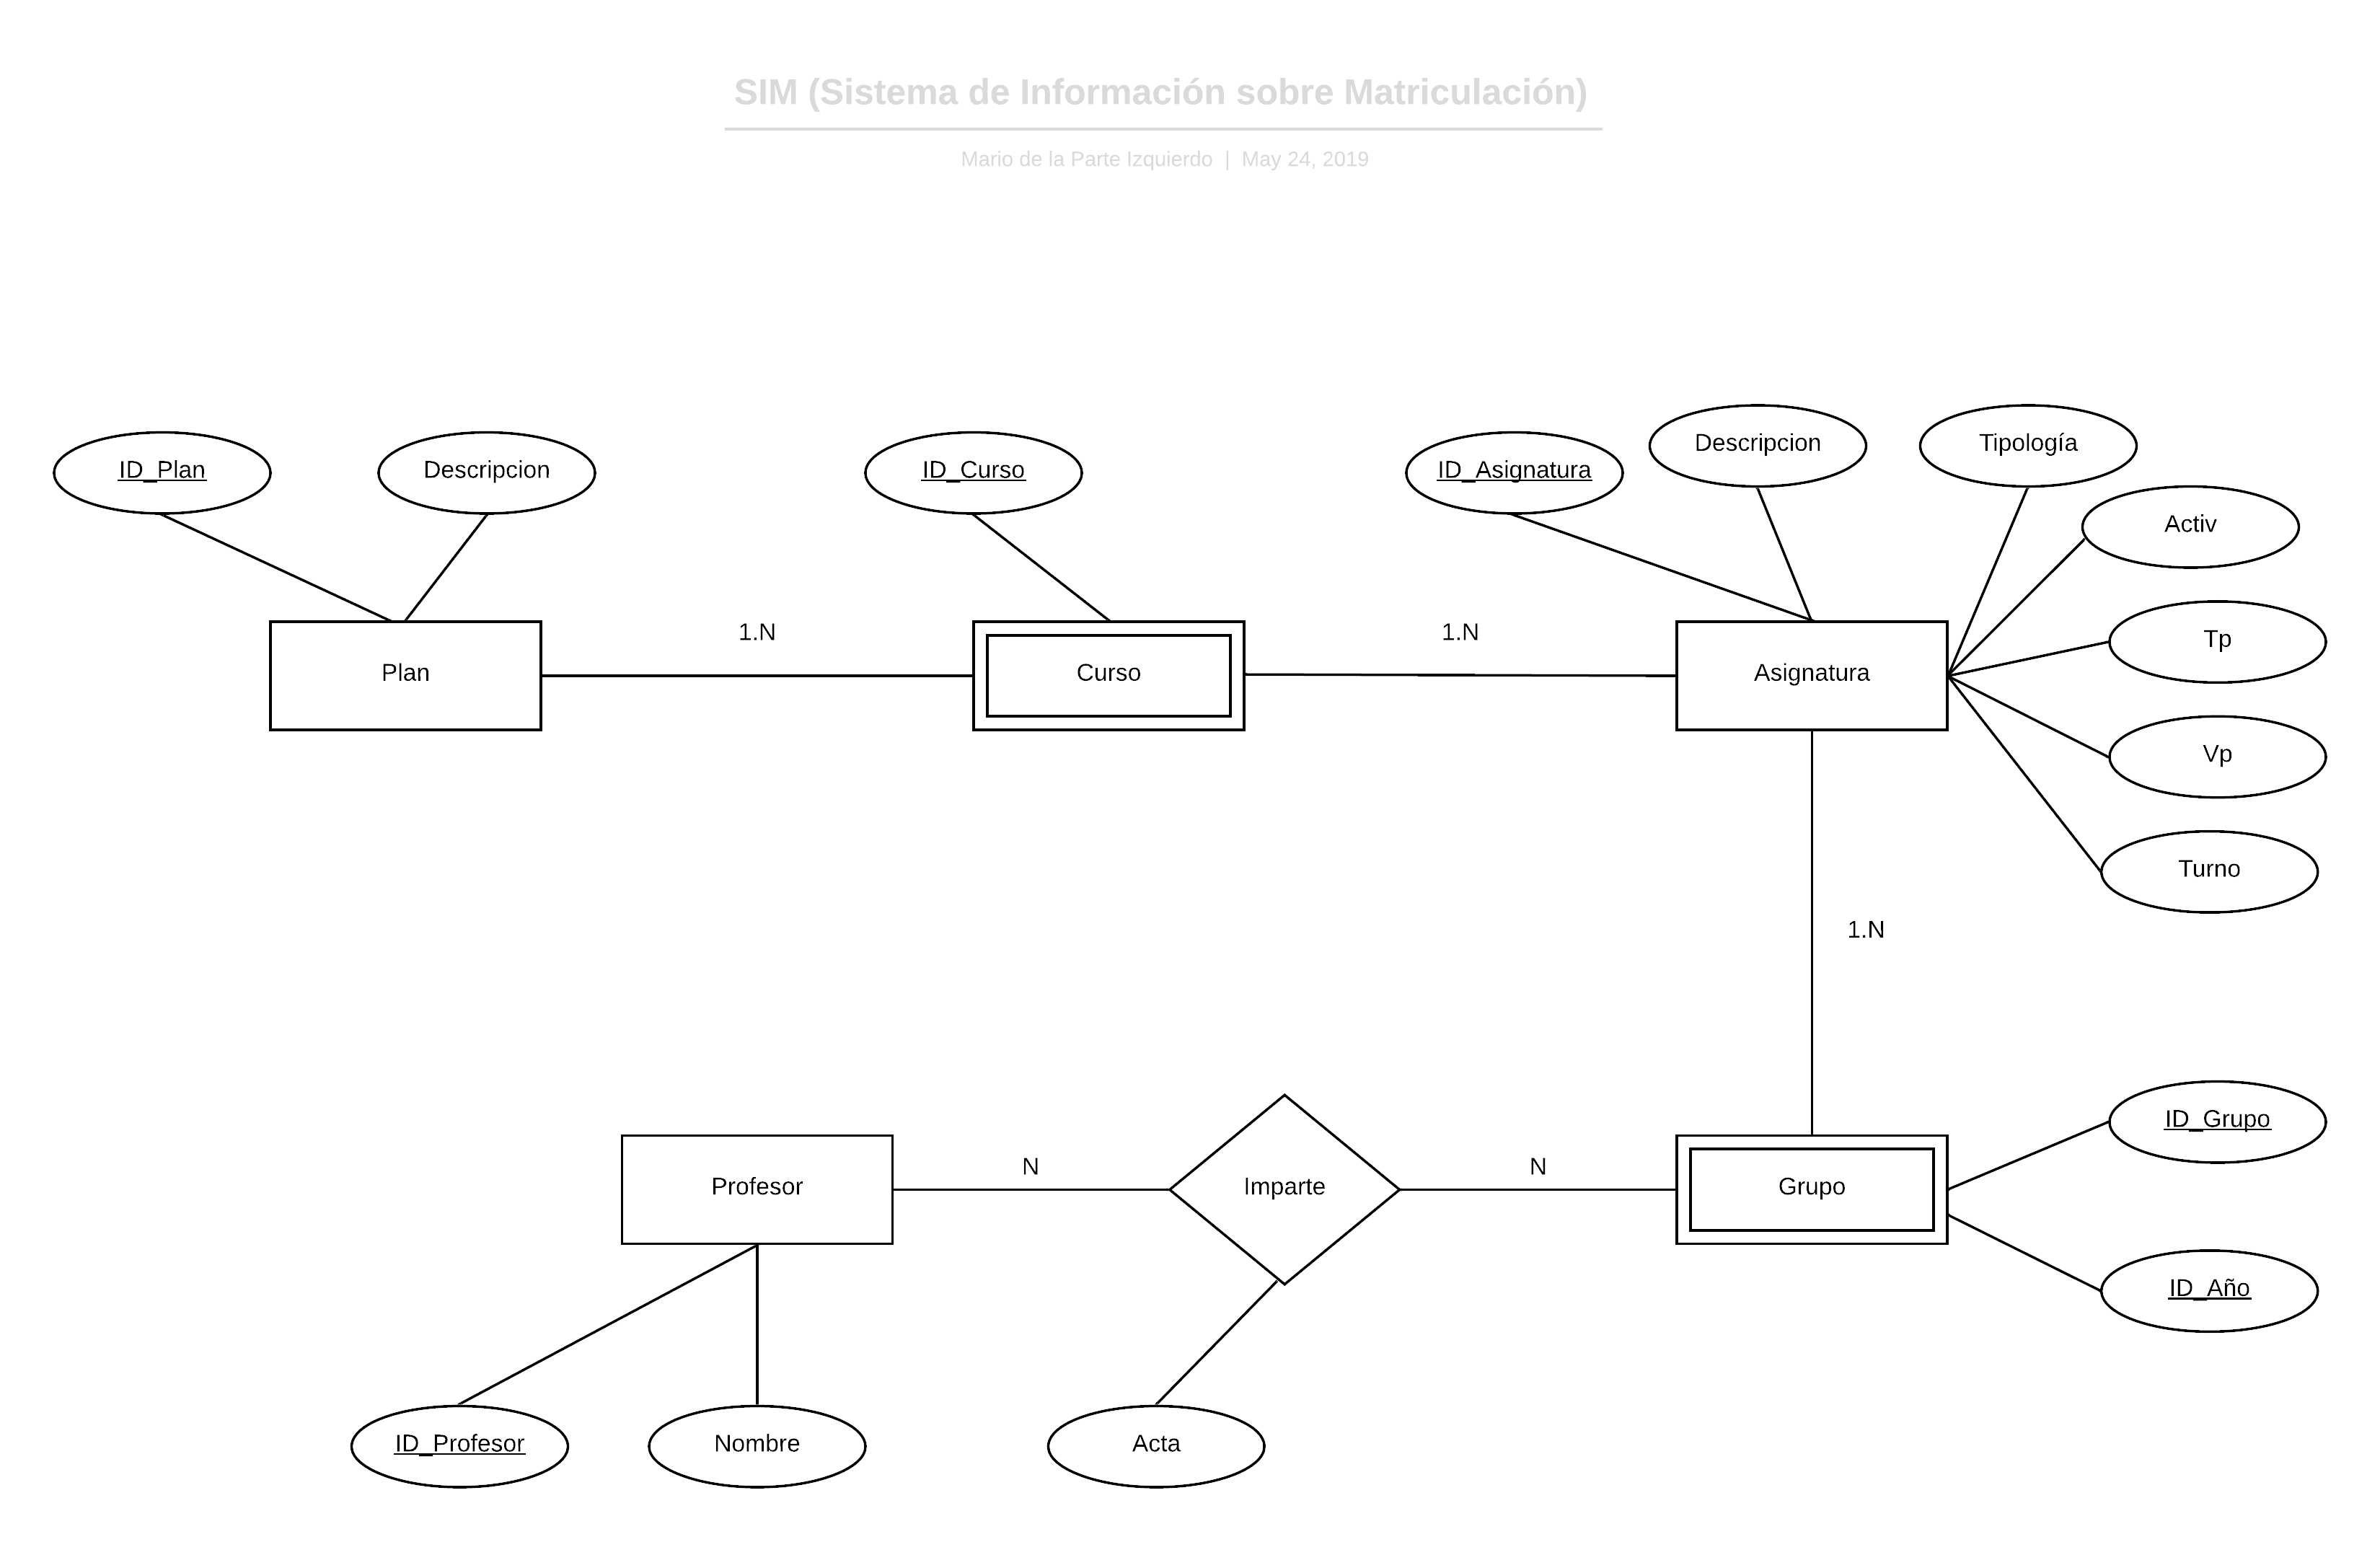
\includegraphics[angle=90, scale = 0.19]{ModeloER}

Se aprecia un total de cinco entidades, dos de las cuales son entidades débiles(\emph{Curso} y \emph{Grupo}). En las relaciones entre entidades se aprecia la cardinalidad entre las mismas, existiendo tres relaciones \emph{1.N} y una relación \emph{N.N} entre \emph{Profesores} y \emph{Grupo}. En cada entidad podemos apreciar sus atributos, así como sus claves primarias(subrayadas).



\subsection{Base de datos}
Se utiliza una base de datos(BBDD) para almacenar toda la información de la aplicación. La BBDD está compuesta por tres tablas principales:


\imagen{TablaASIGNATURAS}{Tabla ASIGNATURAS}

\begin{itemize}
\item
\textbf{ASIGNATURAS}: en esta tabla se almacena la información relacionada con las asignaturas que componen un Plan de Estudios o Titulación determinada. Esta tabla está formada por 9 campos, que son los siguientes:
\begin{itemize}
\item
\textbf{Id\_Asignatura}: es la clave primaria de la tabla y almacena el identificador único de la asignatura. Es un campo numérico de 4 dígitos.
\item
\textbf{Descripcion}: se almacena el nombre de la asignatura. Es un campo de caracteres.
\item
\textbf{Curso}: se almacena el curso al que pertenece la asignatura. Es un campo numérico de 1 dígito.
\item
\textbf{Plan}: se almacena el Plan de Estudios o Titulación al que pertenece la asignatura. Es un campo alfanumérico.
\item
\textbf{Tipologia}: se almacena la tipología del grupo, que puede ser teórica o práctica. Es un campo de caracteres.
\item
\textbf{Activ}: se trata de un campo de caracteres.
\item
\textbf{Tp}: es un campo de caracteres.
\item
\textbf{Vp}: es un campo numérico de 1 dígito. Si es 1 significa que la asignatura es del primer semestre y si es 2 indica que la asignatura se imparte en el segundo semestre.
\item
\textbf{Turno}: indica si el horario es de mañana, de tarde o mezcla de ambos (mixto). Se trata de un campo de caracteres.
\end{itemize}





\imagen{TablaGRUPOS}{Tabla GRUPOS}

\item
\textbf{GRUPOS}: en esta tabla se almacena la información relacionada con los grupos. Hay que destacar que esta tabla se trata de una entidad débil, como se ha visto anteriormente en el modelo de Entidad Relación (ER). Tiene una clave primaria formada por 3 capos (Id\_Asignatura, Id\_Grupo y Temporada (Año)) para poder identificar el total de alumnos matriculados en un grupo de una asignatura, en un año académico en concreto. Esta tabla, por lo tanto, está formada por 4 campos:
\begin{itemize}
\item
\textbf{Id\_Asignatura}: es la clave primaria de la tabla \emph{ASIGNATURAS} y almacena el identificador único de la asignatura. Es un campo numérico de 4 dígitos. Como se ha comentado, es un campo que forma parte de la clave primaria de \emph{GRUPOS}, junto a  Id\_Grupo y Temporada.
\item
\textbf{Id\_Grupo}: es el identificador de grupo y forma parte de la clave primaria junto a  Id\_Asignatura y Temporada. Es un campo numérico de 2 dígitos.
\item
\textbf{Temporada}: indica el año que se cursó o se va a cursar un grupo de una asignatura en concreto y por lo tanto, forma parte de la clave primaria junto a  Id\_Asignatura e Id\_Grupo. Es un campo alfanumérico.
\item
\textbf{Total\_Alumnos}: en este campo se almacena la cantidad de alumnos que hay matriculados en un grupo de una asignatura en un año determinado. Se trata, por tanto, de un campo numérico.
\end{itemize}




\imagen{TablaPROFESORES}{Tabla PROFESORES}

\item
\textbf{PROFESORES}: esta tabla surge de la relación entre las entidades \emph{Grupos} (entidad débil) y \emph{Profesores} como se ha apreciado anteriormente en el modelo Entidad Relación (ER). En esta tabla se almacena la información relacionada con los profesores y los grupos de asignaturas que imparten clase en un año determinado. Tiene una clave primaria formada por 4 campos (Id\_Profesor, Id\_Asignatura, Id\_Grupo y Temporada (Año)). Esta tabla, está formada por estos 6 campos:
\begin{itemize}
\item
\textbf{Id\_Profesor}: forma parte de la clave primaria de la tabla y almacena el identificador único de profesores. Es un campo numérico de 4 dígitos.
\item
\textbf{Id\_Asignatura}: es un campo que forma parte de la clave primaria y almacena el identificador único de la asignatura. Se trata de un campo numérico de 4 dígitos.
\item
\textbf{Id\_Grupo}: es el identificador de grupo y forma parte de la clave primaria. Es un campo numérico de 2 dígitos..
\item
\textbf{Temporada}: indica el año en el que un determinado profesor impartió un grupo de una asignatura. Por lo tanto, forma parte de la clave primaria y es un campo alfanumérico.
\item
\textbf{Acta}: se almacena la información relevante sobre si el profesor firma o no el acta. Es un campo de caracteres.
\item
\textbf{Nombre\_Apellidos}: es un campo que almacena el nombre y apellidos de un profesor. Se trata de un campo de caracteres.
\end{itemize}

\end{itemize}




\section{Diseño procedimental}

Para entender mejor el comportamiento de la aplicación, en la figura \ref{fig:diagramaNav} se puede apreciar el diagrama de navegabilidad de la aplicación.
En dicho diagrama se pueden observar los diferentes procedimientos o funcionalidades que existen en el proyecto. Por lo general, se ha tratado de crear una función por cada una de las cajas representadas en el diagrama anterior, pero en algún caso no ha sido posible y se ha dividido en dos o más funciones, por tratarse de procesos más complejos. A continuación se enumeran las funciones más relevantes del proyecto:

\begin{itemize}

\item \textbf{preprocesar.} Función que se encarga de convertir los (.xls) corruptos que seleccionemos en ficheros (.csv)
para su posterior carga en la BBDD. Para esta labor, llama a la función algoritmo pasándole el nombre del archivo selecionado 
por el usuario con anterioridad.

\item \textbf{algoritmo.} Es una de las funciones más complejas de la aplicación, y realiza las siguientes funciones:
	\begin{itemize}
    \item 1. Abrir un fichero Excel (.xls) como si fuera un (.txt), para obtener un (.xml).
    \item 2. Parsear el contenido del (.xml) y obtener toda la información del Excel(todas las celdas).
       \begin{itemize} 
       \item 2.1. Se obtiene toda la información de cada fila del Excel -> ROW.
        \item 2.2. Se obtiene toda la información de cada celda del Excel -> CELL.
        	 \begin{itemize} 
              \item  2.2.1. Se obtienen los valores MergeDown y MergeAcross de cada celda.
            \end{itemize}
        \end{itemize}  
     \item   2.3. Se obtiene la información \emph{visual}  de cada celda -> DATA.
    3. Con toda la información anterior, se crea un fichero (.csv) y se va guardando la información correctamente.
    \end{itemize}
    

\item \textbf{crearBBDD.} Función que se encarga de la creación de la Base de Datos. Crea una Base de Datos llamada \emph{BBDD} con 3 tablas: ASIGNATURAS, GRUPOS y PROFESORES. Si ya existiera creada la Base de Datos \emph{BBDD} muestra una ventana de tipo warning mostrando por pantalla el mensaje: \emph{La BBDD ya está creada}.



\item \textbf{funcionCargar.} Función que se encarga de: 
	\begin{itemize}
     \item 1. Mostrar una ventana del sistema operativo que nos permite seleccionar archivos.
    \item  2. Una vez seleccionado un archivo, obtiene el nombre y se lo pasa a la función \emph{cargarDatos}, para que devuelva un dataframe con todos los datos.
     \item 3. Se rellenan los datos en las 3 tablas de la BBBD, llamando a las funciones \emph{addAsignaturasRows}, \emph{addGruposRows} y \emph{addProfesoresRows}. 
     \item 4. También se llama a la función \emph{obtenerTemporada}, ya que es la única forma de recuperar u obtener dicho valor.
	\end{itemize}

\item \textbf{cargarDatos.} Función que se encarga de abrir el fichero que se le pasa por parámetro (ruta), siempre y cuando, este fichero se encuentre en el directorio donde nos encontremos. Devuelve un dataFrame con todos los datos del fichero (SIN CONTAR LAS 4 PRIMERAS FILAS DE DATOS).

\item \textbf{ventanaGrafica1.} Función que se encarga de generar la ventana secundaria para posteriormente poder personalizar, generar y descargar el tipo de Gráfico 1.
	\begin{itemize}
    \item 1. Se crea la ventana \emph{hija} raiz2 con las mismas características que la ventana principal.
    \item 2. Se realizan consultas a la BBDD para poder rellenar la información a mostrar en los diferentes desplegables.
    \item 3. Cada vez que se selecciona una opción en los desplegables, se actualiza el valor de la variable global que almacena dicho valor.
    \item 4. Finalmente se cuenta con 2 botones (\emph{Salir} y \emph{Descargar Gráfica}). El segundo llama a la función \emph{descargarG1} para que se proceda a la descarga.
	\end{itemize}
	

\item \textbf{descargarG1.} Función que se encarga de generar y descargar el tipo de Gráfico 1 en función de las opciones que el usuario seleccione en los desplegables.
	\begin{itemize}
    \item 1. Se realiza una consulta a la BBDD en función a los datos seleccionados por el usuario 
    \item 2. Se genera el gráfico, agrupando correctamente los datos anteriormente devueltos, así como personalizando el gráfico (tipo, ejes, nombres, tamaños...etc).
    \item 3. Se descarga el gráfico con el nombre generado con los parámetros seleccionados por el usuario.
	\end{itemize}


\item \textbf{ventanaGrafica2 y ventanaGrafica3.} Funciones muy parecidas a ventanaGrafica1, teniendo la particularidad de que además de llamar a descargarG2 y descargarG3 respectivamente, llaman a rellenarListaG2 y rellenarListaG3. Estas funciones se encargan de hacer consultas a la BBDD en función de los parámetros que se le pasen por cabecera y devuelven una lista con el número de matriculados en las asignaturas del curso que se le pase por parámetro.

\item \textbf{obtenerTemporada.} Función que se encarga de abrir el fichero que se le pasa por parámetro, siempre y cuando, este fichero se encuentre en el directorio donde nos encontremos; y devuelve el valor del año académico de la titulación/plan del fichero.

\item \textbf{addAsignaturasRows, addGruposRows y addProfesoresRows.} Son funciones que se encargan de añadir los datos necesarios del dataframe y de la temporada que se le pasa por parámetro a la tabla determinada de la BBDD.

\item \textbf{hacer\_consulta.} Función que se encarga de realizar consultas a la Base de Datos. Realiza la consulta que se le pase por parámetro (consulta) y devuelve un cursor con el resultado de la misma.

\item \textbf{abrirArchivo.} Función que se encarga de abrir y visualizar el archivo que se le pasa por parámetro.

\end{itemize}

Hay que destacar que para la creación del menú superior de la aplicación, se utiliza una clase denominada \emph{menuSuperior}, con las siguientes funciones:
\begin{itemize}
\item \textbf{abrirAyudaWeb.}
\item \textbf{abrirAbout.}
\item \textbf{abrirAyudaLocal.}
\end{itemize}

\begin{figure}%[!h]
		\centering
		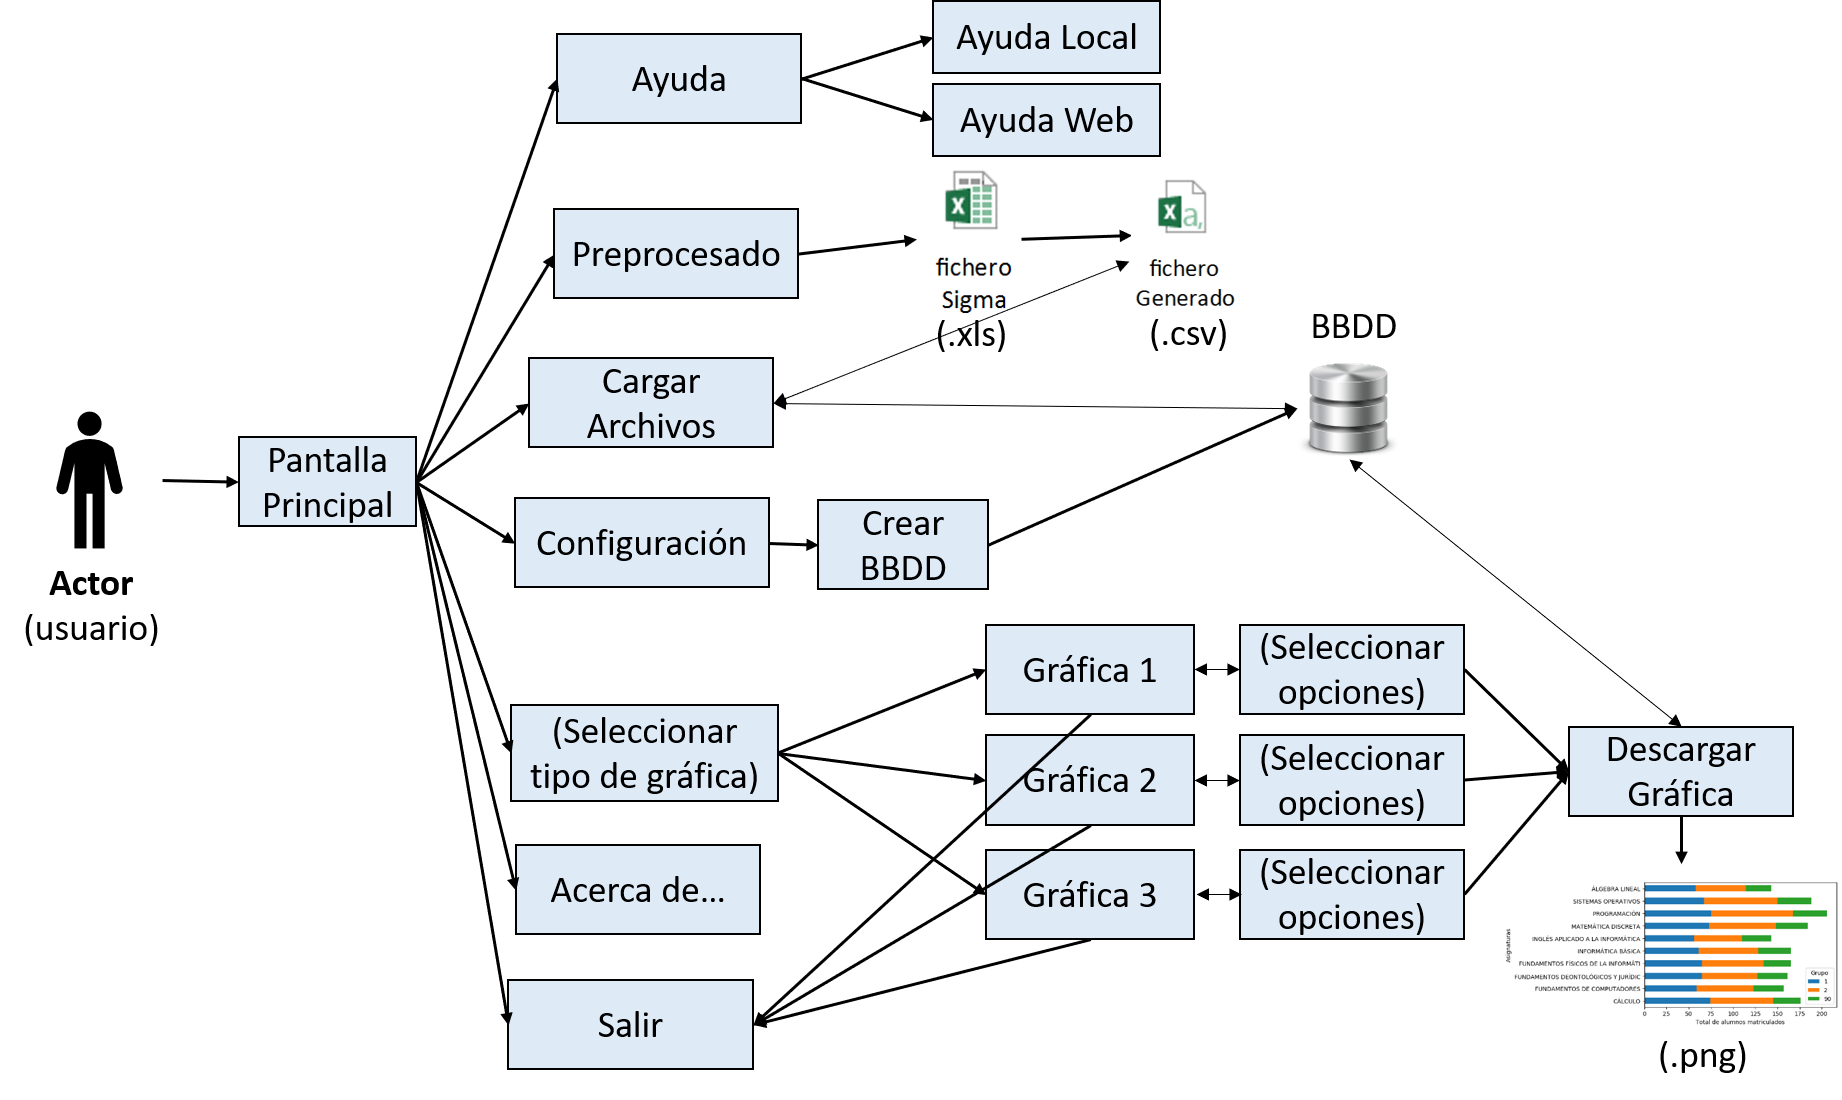
\includegraphics[angle=90, width=\textwidth]{diagramaNav}
		\caption{Diagrama de Navegabilidad}\label{fig:diagramaNav}
	\end{figure}
	

%\section{Diseño arquitectónico}



\section{Diseño de interfaces}

Para el diseño de la interfaz de usuario, el objetivo principal era el de dotar de funcionalidad y sencillez a la aplicación. Se ha conseguido crear  una interfaz funcional, limpia y clara para facilitar la interacción con el usuario.
Esto se ha logrado en parte gracias a la librería \emph{tkinter} de \emph{Python}, ya que se caracteriza por su funcionalidad y utilidad, en contra del aspecto visual o el orientado hacia el diseño gráfico.

A continuación, en la figura \ref{fig:pantallaPrincipal2}, se muestra la vista de la ventana principal de la aplicación. En la figura se puede apreciar que se trata de una interfaz muy sencilla, sin imágenes ni fondos intrusivos.

\begin{figure}%[!h]
		\centering
		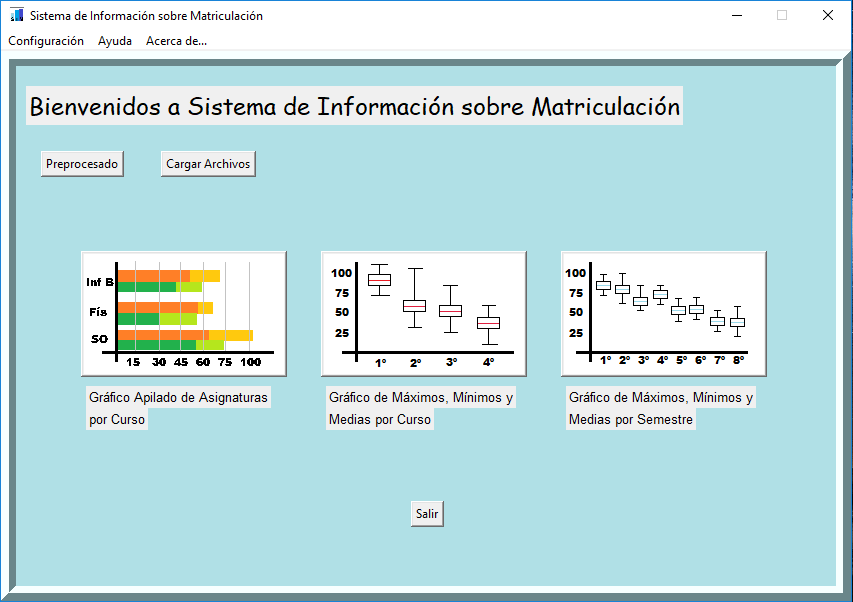
\includegraphics[width=\textwidth]{pantallaPrincipal2}
		\caption{Pantalla principal de la interfaz}\label{fig:pantallaPrincipal2}
	\end{figure}	

Con la finalidad de mejorar la experiencia del usuario se han incorporado una serie de características o mejoras en la interfaz.

Cuando se quiere informar de algún acontecimiento relevante al usuario, se le muestran ventanas emergentes, con la finalidad de captar la atención del mismo. 
Estas ventanas emergentes, pueden ser de tipo \emph{Warning} como la figura \ref{fig:warningBBDD} o simplemente informativas como se aprecia en la figura \ref{fig:salir}

\begin{figure}%[!h]
		\centering
		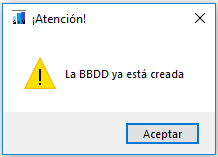
\includegraphics[width=0.4\textwidth]{warningBBDD}
		\caption{Ventana emergente de tipo Warning de la interfaz}\label{fig:warningBBDD}
	\end{figure}
	
\begin{figure}%[!h]
		\centering
		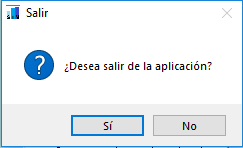
\includegraphics[width=0.4\textwidth]{salir}
		\caption{Ventana emergente informativa de la interfaz}\label{fig:salir}
	\end{figure}
	
Para evitar errores o confusiones, cuando se muestran ventanas propias del sistema operativo, como es el caso de la figura \ref{fig:ventanaSOcsv}, se indica en la parte superior de la ventana un mensaje explicando qué tipos de archivos hay que seleccionar.

Adicionalmente, como se puede apreciar en la figura \ref{fig:ventanaSOcsv},en la parte inferior sólo nos deja seleccionar el tipo de archivos necesarios (en este caso .csv), evitando así la subida de ficheros no válidos. Además, en el tipo de archivos nos muestra el mensaje \emph{.csv (Ya parseados)}, para comprender con mayor facilidad, el tipo de archivos que hay que seleccionar.
	
\begin{figure}%[!h]
		\centering
		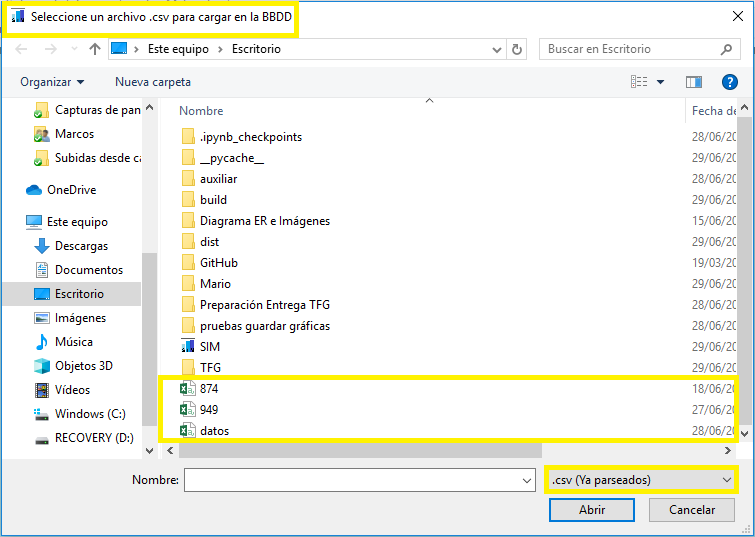
\includegraphics[width=0.9\textwidth]{ventanaSOcsv}
		\caption{Textos de ayuda en la selección de archivos}\label{fig:ventanaSOcsv}
	\end{figure}
		
	
En las pantallas secundarias (pantallas de los diferentes tipos de gráficos), se muestra en la parte superior migas de pan o \emph{breadcrumb-trail} como se aprecia en la figura  \ref{fig:migasDePan} .

\begin{figure}%[!h]
		\centering
		
\includegraphics[width=0.9\textwidth]{migasDePan}
		\caption{Migas de pan de la ventana secundaria}\label{fig:migasDePan}
	\end{figure}
	
	
	